\documentclass{beamer}
\usetheme{Boadilla}
\usepackage{tikz}
\usepackage{graphicx}
\usepackage{amsmath}




\title{Weekly Presentation}
\subtitle{Week 40}
\author{}
\institute{Luleå University of Technology}
\date{\today}



\begin{document}
\begin{frame}
    \titlepage
\end{frame}


%%%%%%%%%%%%%%%% new page %%%%%%%%%%%%%%%%%%%%%%


\begin{frame}
    \subsection{Group members}
    \frametitle{Group members }
    \begin{itemize}
        \item Y-students
        \begin{itemize}
            \item Martin Blaszczyk - Project leader and object detection
            \item Edward Cedergård -Arm and gripping tool
            \item Niklad Dahlqvist -  Arm and gripping tool
            \item Måns Norell - Movable base
        \end{itemize}
        \item D-students
        \begin{itemize}
            \item Edward Källstedt - Object detection
            \item Albin Martinsson - Arrowhead and Git
        \end{itemize}  
    \end{itemize}
\end{frame}


%%%%%%%%%%%%%%%% new page %%%%%%%%%%%%%%%%%%%%%%


\begin{frame}{Overview}
What we have done and what we are working on:
    \begin{itemize}
        \item Full duplex to half duplex serial communication
        \item Dynamixel data packages
    \end{itemize}
\end{frame}



%%%%%%%%%%%%%%%% new page %%%%%%%%%%%%%%%%%%%%%%




%%%%%%%%%%%%%%%% new page %%%%%%%%%%%%%%%%%%%%%%

\begin{frame}{Full-duplex to half-duplex }

    \begin{figure}
        \centering
        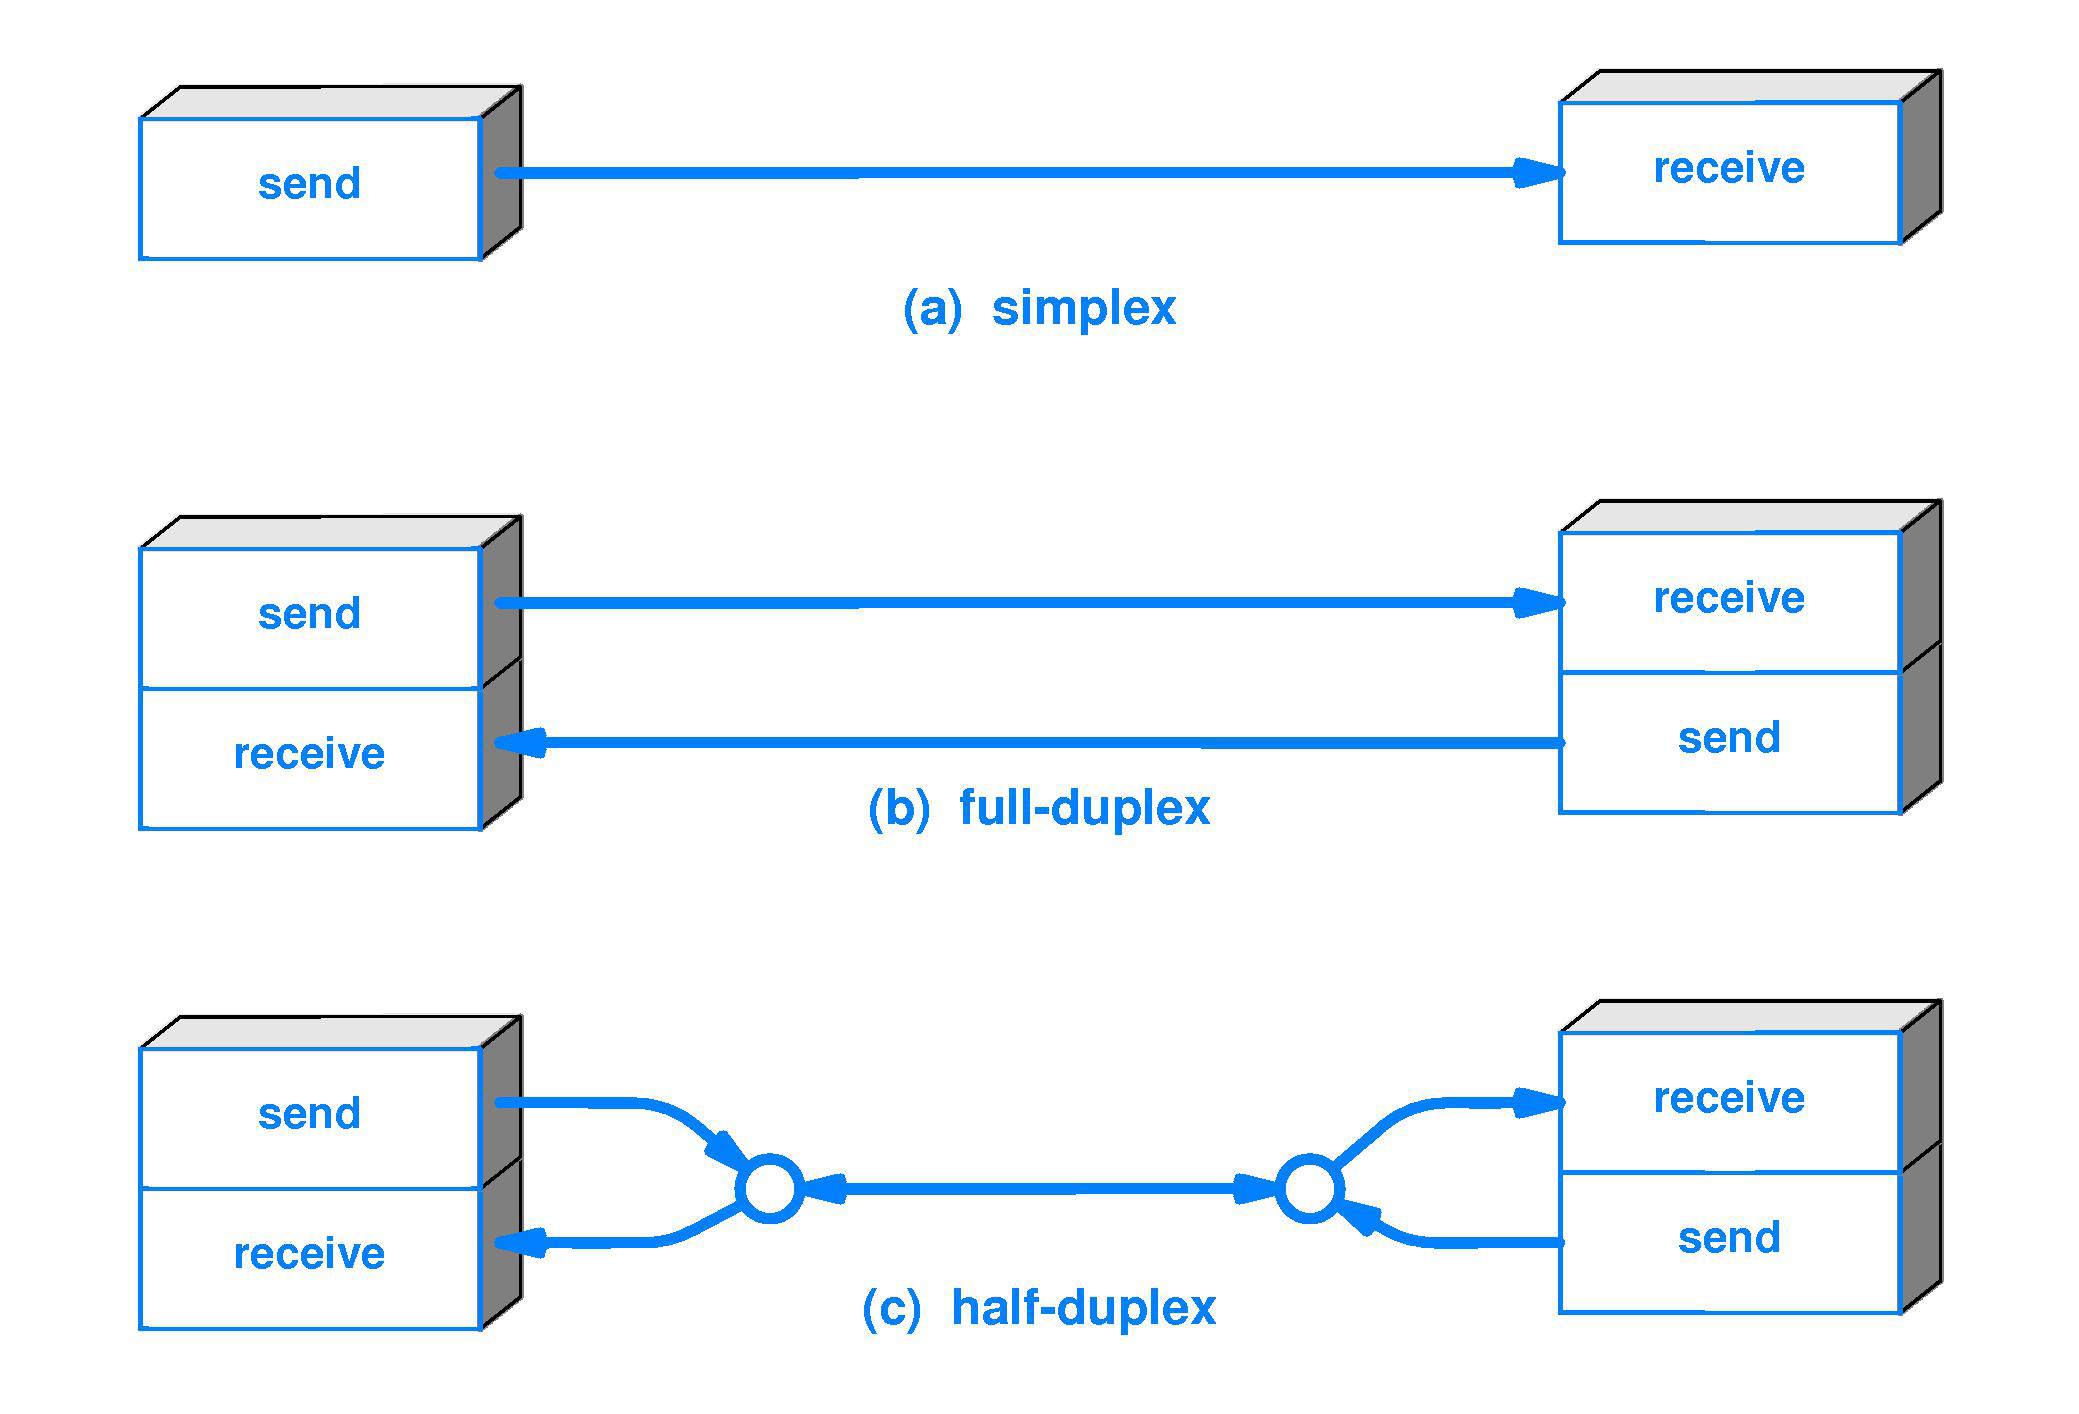
\includegraphics[width = \textwidth]{img/BBE_Simplex vs Duplex_Transmissions.jpg}
        
    \end{figure}
    
\end{frame}


%%%%%%%%%%%%%%%% new page %%%%%%%%%%%%%%%%%%%%%%

\begin{frame}{Dynamixel communication}

    \begin{figure}
        \centering
        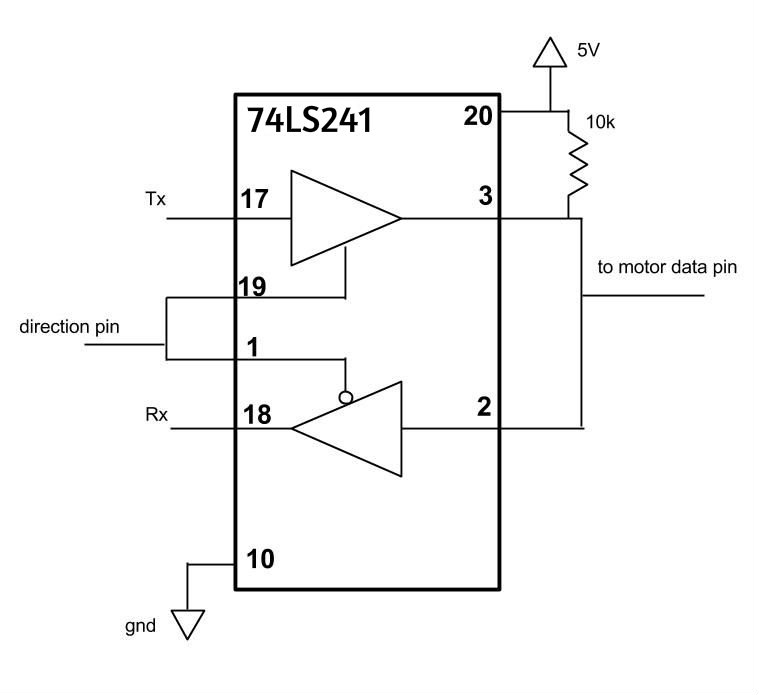
\includegraphics[width =9.5cm]{img/uart_half-duplex_74LS241.jpg}
        
    \end{figure}
    
\end{frame}


%%%%%%%%%%%%%%%% new page %%%%%%%%%%%%%%%%%%%%%%

\begin{frame}{Curcuit}

    \begin{figure}
        \centering
        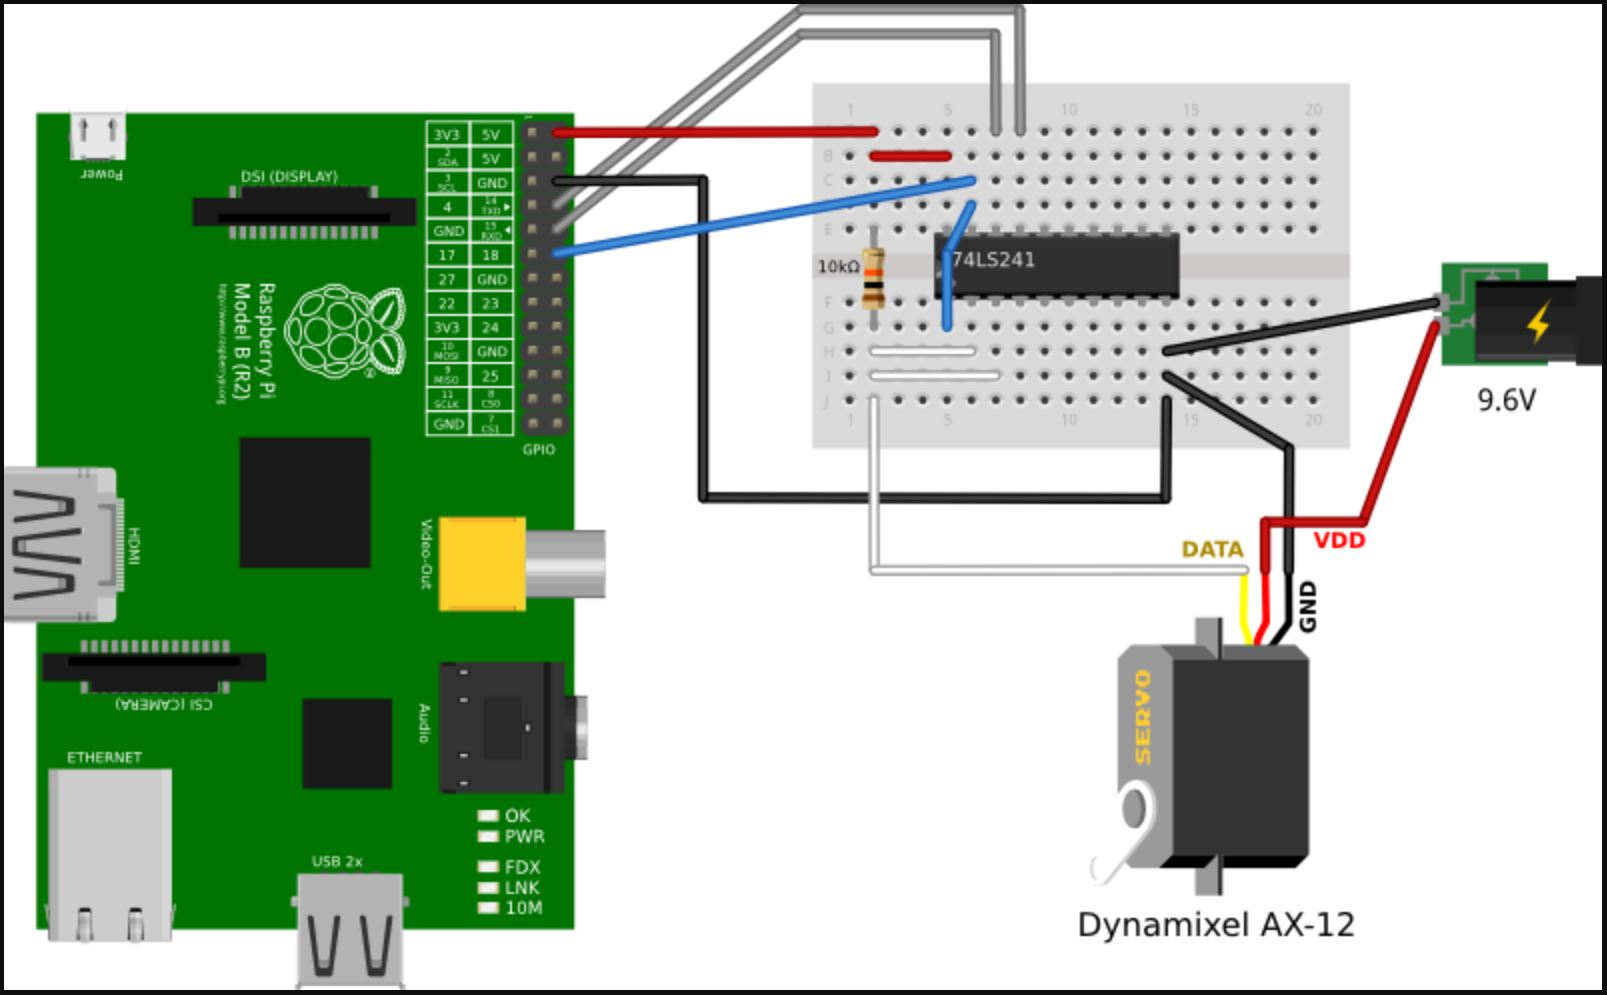
\includegraphics[width = \textwidth]{img/circuit.png}
    \end{figure}
    
\end{frame}




%%%%%%%%%%%%%%%% new page %%%%%%%%%%%%%%%%%%%%%%


\begin{frame}{Dynamixel data packages overview}

    \begin{columns}
        \begin{column}[]{0.5\textwidth}
            \begin{itemize}
                \item Data packets structure
                \item Timing of response
                \item Example package
            \end{itemize}
        \end{column}
        
        
        \begin{column}[]{0.5\textwidth}
        \end{column}
    \end{columns}
    
\end{frame}

%%%%%%%%%%%%%%%% new page %%%%%%%%%%%%%%%%%%%%%%


\begin{frame}{Dynamixel data packages}

    Instruction package - send to the motor

    \begin{table}
        \begin{tabular}{| c | c | c | c | c | c | c | c |}
            \hline
            Header & ID & Length & Instruction & Param 1 & ... & n & Checksum\\
            \hline
            0xFFFF & ID & Length & Instruction & param 1 & ... & n & Checksum\\
            \hline
        \end{tabular}
    \end{table}
    
    Status return package - recieve from the motor

    \begin{table}
        \begin{tabular}{| c | c | c | c | c | c | c | c |}
            \hline
            Header & ID & Length & Error & Param 1 & ... & n & Checksum\\
            \hline
            0xFFFF & ID & Length & Error & Param 1 & ... & n & Checksum\\
            \hline
        \end{tabular}
    \end{table}
    
\end{frame}


%%%%%%%%%%%%%%%% new page %%%%%%%%%%%%%%%%%%%%%%


\begin{frame}{Instruction package}
    
        \begin{table}
            \begin{flushleft}
                \begin{tabular}{| c |}
                    \hline
                    Header\\
                    \hline
                    0xFFFF\\
                    \hline
                \end{tabular}
            \end{flushleft}
        \end{table}

        Header allways fixed.

\end{frame}

%%%%%%%%%%%%%%%% new page %%%%%%%%%%%%%%%%%%%%%%


\begin{frame}{Instruction package}
 
    \begin{table}
        \begin{flushleft}
            \begin{tabular}{| c | c |}
                \hline
                Header & ID\\
                \hline
                0xFFFF & ID\\
                \hline
            \end{tabular}
        \end{flushleft}
    \end{table}

    ID is a unique number for each motor connected.
    
\end{frame}


%%%%%%%%%%%%%%%% new page %%%%%%%%%%%%%%%%%%%%%%


\begin{frame}{Instruction package}
 
    \begin{table}
        \begin{flushleft}
            \begin{tabular}{| c | c | c |}
                \hline
                Header & ID & Length\\
                \hline
                0xFFFF & ID & Length \\
                \hline
            \end{tabular}
        \end{flushleft}
    \end{table}

    Length of the message, excluding the header bytes.
    
\end{frame}



%%%%%%%%%%%%%%%% new page %%%%%%%%%%%%%%%%%%%%%%


\begin{frame}{Instruction package}
 
    \begin{table}
        \begin{flushleft}
            \begin{tabular}{| c | c | c | c | c | c | c |}
                \hline
                Header & ID & Length & Instruction & Param 1 & ... & Param n\\
                \hline
                0xFFFF & ID & Length & Instruction & param 1 & ... & Param n\\
                \hline
            \end{tabular}
        \end{flushleft}
    \end{table}

    Parameters, depends on the instruction.
    
\end{frame}


%%%%%%%%%%%%%%%% new page %%%%%%%%%%%%%%%%%%%%%%


\begin{frame}{Instruction package}

    \begin{table}
        \begin{flushleft}
            \begin{tabular}{| c | c | c | c | c | c | c | c |}
                \hline
                Header & ID & Length & Instruction & Param 1 & ... & n & Checksum\\
                \hline
                0xFFFF & ID & Length & Instruction & param 1 & ... & n & Checksum\\
                \hline
            \end{tabular}
        \end{flushleft}
    \end{table}

    The checksum is calculated as\\
    Checksum = ~( ID + Length + Instruction + Parameter1 + … Parameter N )\\
    where "" is the "not" operation and only the lower byte is used.
\end{frame}

%%%%%%%%%%%%%%%% new page %%%%%%%%%%%%%%%%%%%%%%


\begin{frame}{Status return package}

    \begin{table}
        \begin{flushleft}
            \begin{tabular}{| c | c | c | c | c | c | c | c |}
                \hline
                Header & ID & Length & Error & Param 1 & ... & Param n & Checksum\\
                \hline
                0xFFFF & ID & Length & Error & Param 1 & ... & Param n & Checksum\\
                \hline
            \end{tabular}
        \end{flushleft}
    \end{table}
    Similar to instruction package but each bit in the error byte represents one possible error.
    
\end{frame}

%%%%%%%%%%%%%%%% new page %%%%%%%%%%%%%%%%%%%%%%


\begin{frame}{Timing of return package}

    \begin{itemize}
        \item Return delay can be set for each motor
        \item Values between 0 - 508 microseconds
    \end{itemize}
    
\end{frame}



%%%%%%%%%%%%%%%% new page %%%%%%%%%%%%%%%%%%%%%%


\begin{frame}{Example package}

    \begin{table}
        \begin{flushleft}
            \begin{tabular}{| c | c | c | c | c | c | c | c |}
                \hline
                Header & ID & Length & Instr. & P.1 & P.2 & P.3 & Checksum\\
                \hline
                0xFFFF & 0x01 & 0x04 & 0x03 & 0x1E & 0x00 & 0x00 & 0xD9\\
                \hline
            \end{tabular}
        \end{flushleft}
    \end{table}
    Writes the data 0x0000 at memory position 0x1E. (Goal position = 0)
\end{frame}

%%%%%%%%%%%%%%%% new page %%%%%%%%%%%%%%%%%%%%%%


\begin{frame}{Logic analyzer example}


        \begin{figure}
            \centering
            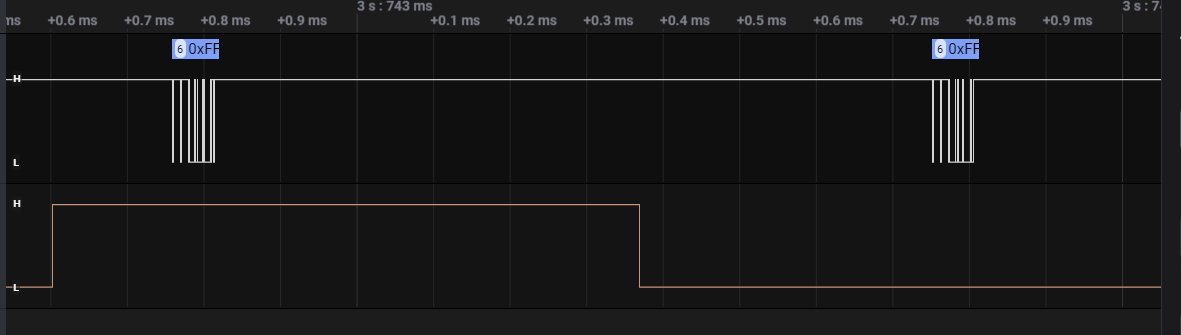
\includegraphics[width = \textwidth]{img/logic_1.PNG}

        \end{figure}
    
\end{frame}


%%%%%%%%%%%%%%%% new page %%%%%%%%%%%%%%%%%%%%%%


\begin{frame}{Logic analyzer example}

    \begin{figure}
        \centering
        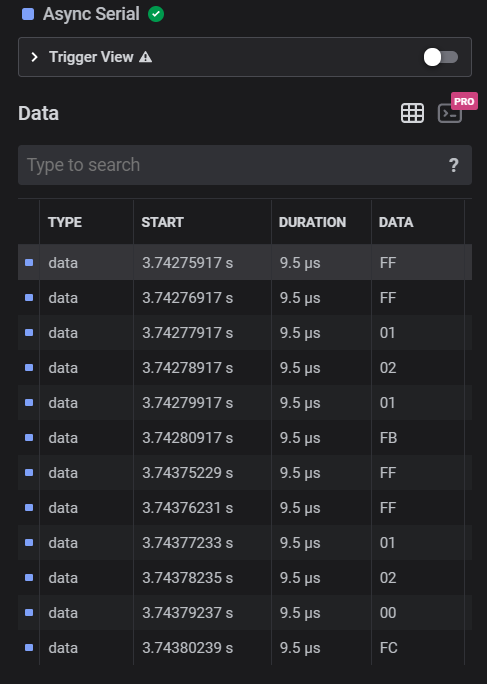
\includegraphics[width = 0.5\textwidth]{img/logic_2.PNG}

    \end{figure}

\end{frame}


%%%%%%%%%%%%%%%% new page %%%%%%%%%%%%%%%%%%%%%%



\begin{frame}{Demonstration}


        \begin{itemize}
            \item \url{https://youtu.be/f_JAT8srcIc}
        \end{itemize}

    
\end{frame}

%%%%%%%%%%%%%%%% new page %%%%%%%%%%%%%%%%%%%%%%



\begin{frame}{Additional information}


    \begin{itemize}
        \item \url{https://emanual.robotis.com/docs/en/dxl/ax/ax-12a/}
        \item \url{https://emanual.robotis.com/docs/en/dxl/protocol1/}
        \item \url{http://www.crustcrawler.com/products/bioloid/docs/AX-12.pdf}
    \end{itemize}


\end{frame}


%%%%%%%%%%%%%%%% new page %%%%%%%%%%%%%%%%%%%%%%



%%%%%%%%%%%%%%%% new page %%%%%%%%%%%%%%%%%%%%%%



%\begin{frame}
%   \titlepage
%\end{frame}


%%%%%%%%%%%%%%%% new page %%%%%%%%%%%%%%%%%%%%%%


\begin{frame}{Movable Base}
What has been done\\
\begin{itemize}
    \item CAD model for base have been made
    \item Controllers have been made to move the base to a specific point in space
    \item Real world limitations have been applied to the controllers
\end{itemize}
\end{frame}



%%%%%%%%%%%%%%%% new page %%%%%%%%%%%%%%%%%%%%%%


\begin{frame}{CAD Model}
\begin{columns}
\begin{column}[]{0.5\textwidth}
THIS IS NOT THE FINAL BASE MODEL\\
It's for prototyping and is modelled to be modular and easy to attach parts to

\end{column}
\begin{column}[]{0.5\textwidth}
\begin{figure}
    \centering
    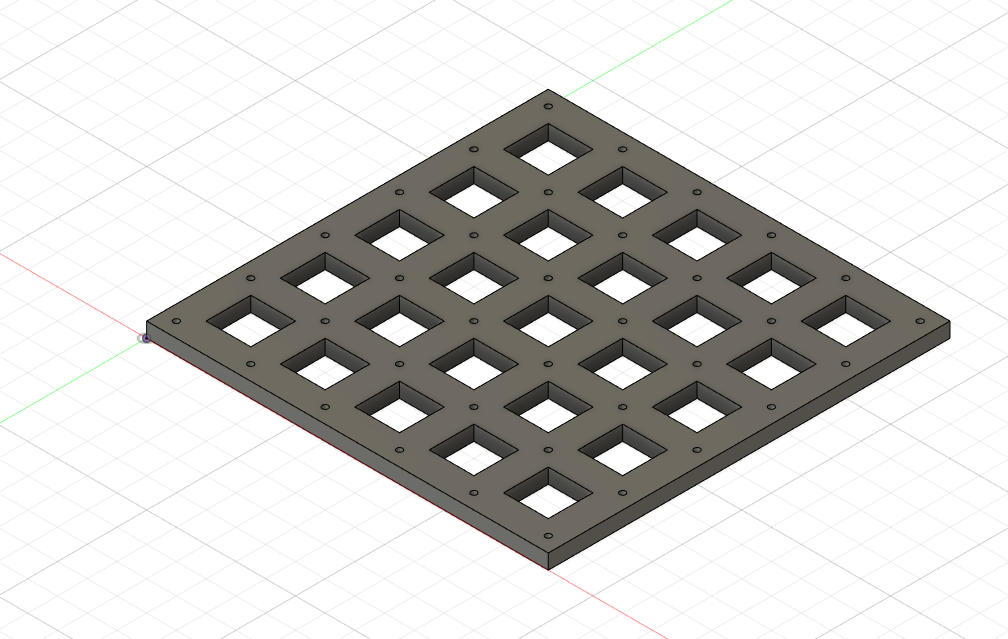
\includegraphics[width=0.5\textwidth]{img/manbase.png}
    \caption{Model of base}
    \label{fig:my_label}
\end{figure}
\end{column}
\end{columns}
\end{frame}


%%%%%%%%%%%%%%%% new page %%%%%%%%%%%%%%%%%%%%%%


\begin{frame}{New Controllers}
Two \textbf{PID} controller are made in order to move to a user specific coordinate by
\begin{itemize}
    \item Setting the robot to a specific angle
    \item Move the robot a user defined distanced
\end{itemize}
\end{frame}


%%%%%%%%%%%%%%%% new page %%%%%%%%%%%%%%%%%%%%%%




%%%%%%%%%%%%%%%% new page %%%%%%%%%%%%%%%%%%%%%%

\begin{frame}{Simulations With Limitations}
\begin{columns}
\begin{column}[]{0.5\textwidth}
\begin{figure}
    \centering
    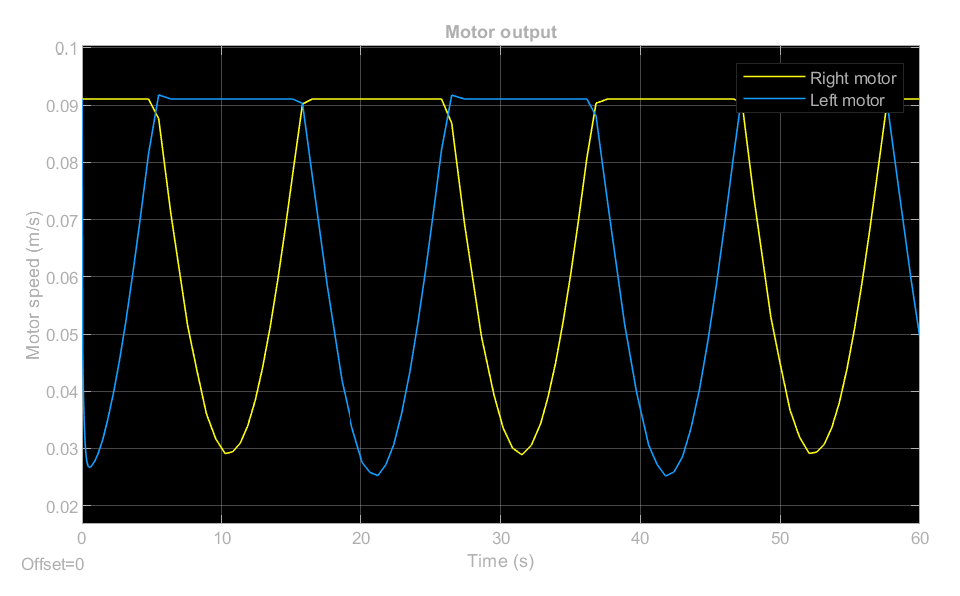
\includegraphics[width=\textwidth]{img/motor_speeds.eps}
    \caption{Motor speeds}
    \label{fig:my_label}
\end{figure}
\end{column}
\begin{column}[]{0.5\textwidth}
\begin{figure}
    \centering
    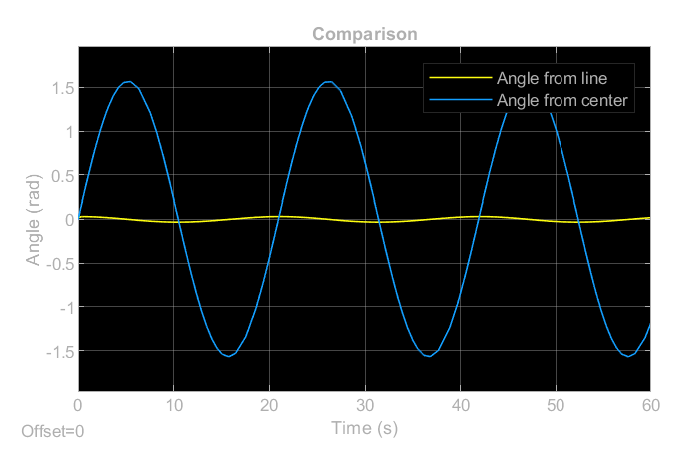
\includegraphics[width=\textwidth]{img/comparison.eps}
    \caption{The angle towards the center and the angle towards the line comparison}
    \label{fig:my_label}
\end{figure}
\end{column}
\end{columns}
    
\end{frame}


%%%%%%%%%%%%%%%% new page %%%%%%%%%%%%%%%%%%%%%%




\begin{frame}{Simulations With Limitations}

\begin{columns}
\begin{column}[]{0.5\textwidth}
\begin{figure}
    \centering
    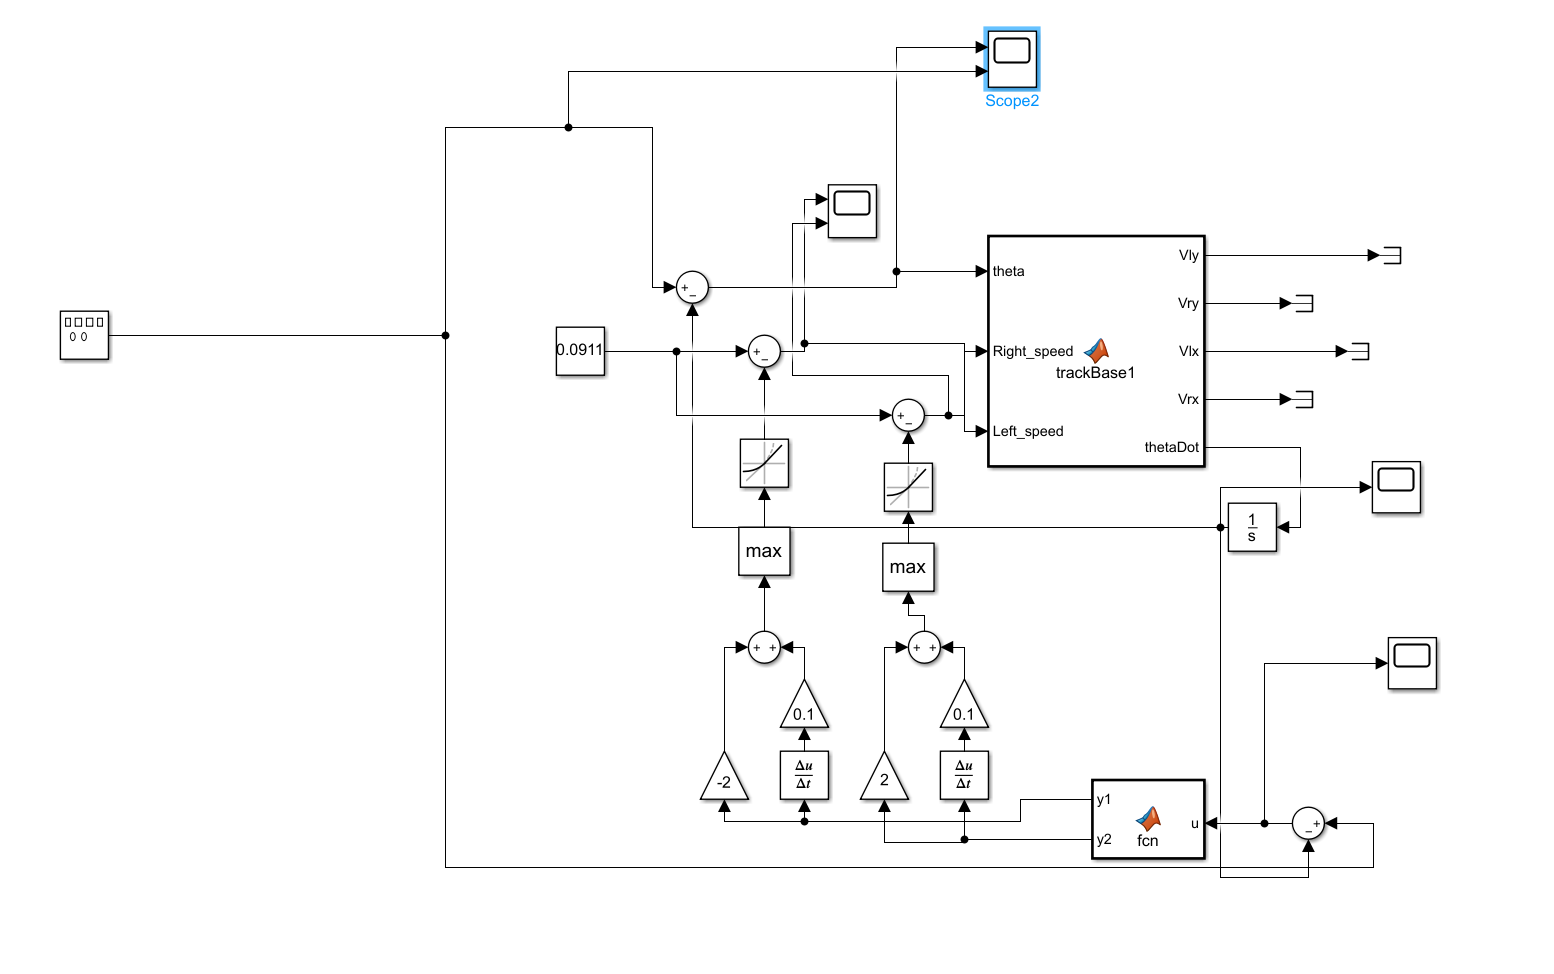
\includegraphics[width=\textwidth]{img/pd_block_diagram.png}
    \caption{Block diagram}
    \label{fig:my_label}
\end{figure}
\end{column}
\begin{column}[]{0.5\textwidth}
\begin{figure}
    \centering
    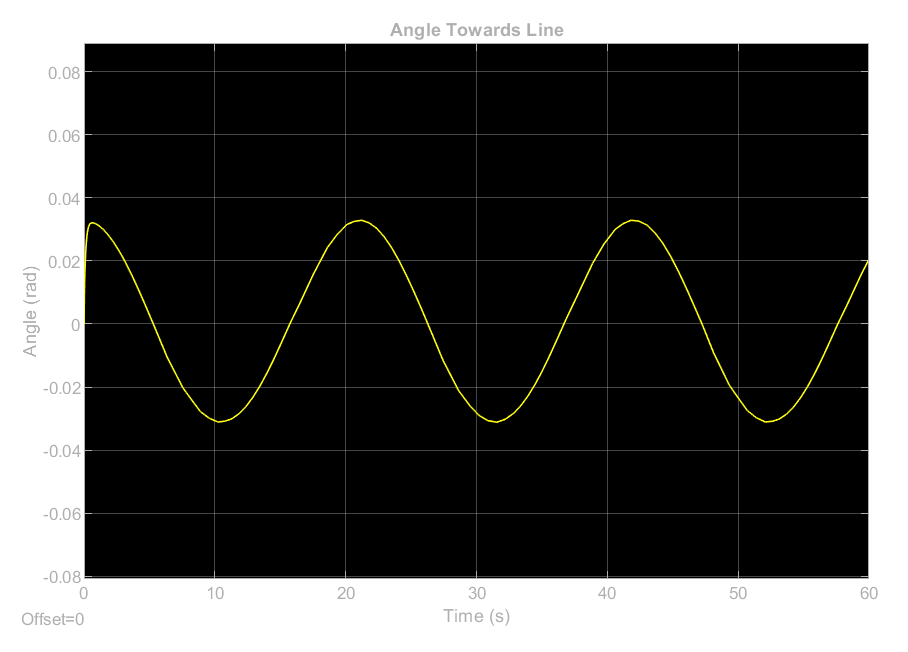
\includegraphics[width=\textwidth]{img/angle_towards_line.eps}
    \caption{The angle towards the line}
    \label{fig:my_label}
\end{figure}
\end{column}
\end{columns}
\end{frame}

\begin{frame}{What Is To Be Done}
    \begin{itemize}
        \item Stability analysis on \textbf{PID}s
        \item 3D print and build robot
        \item Implement controllers on robot
    \end{itemize}
\end{frame}



%%%%%%%%%%%%%%%% new page %%%%%%%%%%%%%%%%%%%%%%


\begin{frame}{Machine Vision Progress}


    \begin{itemize}
        \item Rewritten in C++
        \item Added configuration options
        \item QR-Code detection implemented
    \end{itemize}


\end{frame}

\begin{frame}{Machine Vision Progress}


    \begin{itemize}
        \item \url{https://www.youtube.com/watch?v=b7bSlFM6s4o}
    \end{itemize}


\end{frame}

\begin{frame}{Machine Vision Future Improvements}


    \begin{itemize}
        \item QR detection optimizations
        \item QR orientation
        \item Pathfinding
    \end{itemize}


\end{frame}












%%%%%%%%%%%%%%%% new page %%%%%%%%%%%%%%%%%%%%%%


%%%%%%%%%%%%%%%% new page %%%%%%%%%%%%%%%%%%%%%%




%%%%%%%%%%%%%%%%%%%%%%%%%%%%%%%%%%%%%%%%%%%%%%%%%%%%%%%%%%%%%%%%
%%%%%%%%%%%%%%%%%%%%%%%% Time Plan %%%%%%%%%%%%%%%%%%%%%%%%%%%%%
%%%%%%%%%%%%%%%%%%%%%%%%%%%%%%%%%%%%%%%%%%%%%%%%%%%%%%%%%%%%%%%%
\begin{frame}
    \subsection{Time plan}
    \frametitle{Overall timetable}
    \begin{table}
        \begin{tabular}{| l | c | c | c | c }
            
            Sep & Oct & Nov & Dec \\
            \hline \hline
            Concept generation & Evaluation & Evaluation &  \\ 
            \hline
            Theory & Prototyping & Evaluation & Finishing up \\
            \hline
            Simulation & Evaluation & Evaluation & \\
            \hline
            Prototyping & Final Design & Evaluation &  \\
            \hline
 
        \end{tabular}
    \end{table}    
\end{frame}


\begin{frame}
    \frametitle{Time plan for September}
    \begin{table}
        \begin{tabular}{l | c | c | c | c }
        Subproject & Week 1 & Week 2 & Week 3 & Week 4 \\
        \hline \hline
            Arrowhead & Reading& Setup & API & Prototyping\\
            Movable base & Reading& Modeling & Simulation & Implementation\\
            Arm and grip  & Reading & Kinematics & Simulation& Prototyping\\
            Object detection & Reading & Testing & Prototyping & Evaluation\\
        \end{tabular}
    \end{table}
\end{frame}


\begin{frame}
    \begin{center}
        \Huge Questions?
    \end{center}
\end{frame}



\end{document}
